\section{Introduction}
\begin{figure}[H]
\centering
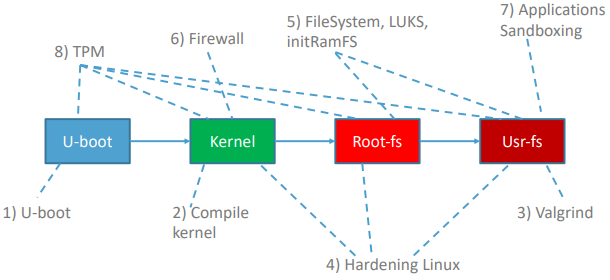
\includegraphics[width=0.8\columnwidth]{cours_struct.png}
\end{figure}
\subsection{Cross-compilation}
Cross-compilation (ARM) effectuée sur un système x86/x64. Buildroot est le toolchain utilisé. Les éléments suivants sont compilés : Bootloader, Kernel, Rootfs. Puis les images sont copiées sur la carte SD